
% Plantilla para la presentación de artículos para el Multicongreso I-D Ingeniería 2014
% Edite el contenido del documento basándose en los lineamientos aqui presentados.
% Esta plantilla es una adaptación que utiliza la clase IEEEtran disponible en:
% http://www.ieee.org/conferences_events/conferences/publishing/templates.html
% No realice modificaciones a los márgenes ni a las propiedades del texto.
% 2014 Universidad de Cuenca
% Asistencia: kenneth.palacio@ucuenca.edu.ec

\documentclass[conference, letterpaper]{IEEEtranMC1}
\usepackage[spanish]{babel}
\usepackage[utf8]{inputenc}
\usepackage{graphicx}

\usepackage{gensymb}
\usepackage{xcolor}
\usepackage{pgfplots}
\usepackage{tikz}

% Define bar chart colors
%
\definecolor{bblue}{HTML}{4F81BD}
\definecolor{rred}{HTML}{C0504D}
\definecolor{ggreen}{HTML}{9BBB59}
\definecolor{ppurple}{HTML}{9F4C7C}
% *** GRAPHICS RELATED PACKAGES ***
%
\ifCLASSINFOpdf
  % \usepackage[pdftex]{graphicx}
  % declare the path(s) where your graphic files are
  % \graphicspath{{../pdf/}{../jpeg/}}
  % and their extensions so you won't have to specify these with
  % every instance of \includegraphics
  % \DeclareGraphicsExtensions{.pdf,.jpeg,.png}
\else
  % or other class option (dvipsone, dvipdf, if not using dvips). graphicx
  % will default to the driver specified in the system graphics.cfg if no
  % driver is specified.
  % \usepackage[dvips]{graphicx}
  % declare the path(s) where your graphic files are
  % \graphicspath{{../eps/}}
  % and their extensions so you won't have to specify these with
  % every instance of \includegraphics
  % \DeclareGraphicsExtensions{.eps}
\fi
% graphicx was written by David Carlisle and Sebastian Rahtz. It is
% required if you want graphics, photos, etc. graphicx.sty is already
% installed on most LaTeX systems. The latest version and documentation can
% be obtained at: 
% http://www.ctan.org/tex-archive/macros/latex/required/graphics/
% Another good source of documentation is "Using Imported Graphics in
% LaTeX2e" by Keith Reckdahl which can be found as epslatex.ps or
% epslatex.pdf at: http://www.ctan.org/tex-archive/info/
%
% latex, and pdflatex in dvi mode, support graphics in encapsulated
%

%
\usepackage{url}

% correct bad hyphenation here
\hyphenation{op-tical net-works semi-conduc-tor}

\begin{document}

%
% paper title
% can use linebreaks \\ within to get better formatting as desired
\title{Coordinación de Arbotix, Raspberry Pi y motores Dynamixel Ax-12+ con el objetivo de la construcción de un robot humanoide que busque  y patee pelotas}

% author names and affiliations
% use a multiple column layout for up to three different
% affiliations


\author{\IEEEauthorblockN{Jennifer Dos Reis}
\IEEEauthorblockA{Grupo De Inteligencia Artificial\\
Universidad Simón Bolívar\\
Caracas, Venezuela\\
08-10323@usb.ve}
\and
\IEEEauthorblockN{Juliana León}
\IEEEauthorblockA{Grupo De Inteligencia Artificial\\
Universidad Simón Bolívar\\
Caracas, Venezuela\\
juliana@ac.labf.usb.ve}
\and
\IEEEauthorblockN{Carolina Chang}
\IEEEauthorblockA{Grupo De Inteligencia Artificial\\
Departamento de Computación y\\ Tecnología de la Información\\
Universidad Simón Bolívar\\
Caracas, Venezuela\\
cchang@usb.ve}
}


% make the title area
\maketitle

\begin{abstractEN}
%\boldmath 

This article presents Debupa (Detección Búsqueda Pateo) a small humanoid (38 cm high) built with the Bioloid Premium Kit \cite{robotics}  from the manufacturer ROBOTIS \cite{robotics1}. The CM-510 card has been excluded to be replaced by the Arbotix controller card, which is used to control the 16 motors Dynamixel AX-12 + (for moving the robot) and 2 analog servo (to move the camera). It has been also added a Raspberry Pi mini computer, with its  camera \cite{raspberry}, so that the robot can detect and track the ball autonomously. 

All these components must be coordinated to accomplish the tasks of detection, tracking and kicking of the ball. Thus, communication between the Arbotix and Raspberry Pi is necessary. The tool used for this is the ROS (Ros Operating System) framework  \cite{ros}.

In the Raspberry Pi the c++ language is used. A program captures the camera image, filters  and processes it  to find the ball, decides the action to take, and  requests the Arbotix  to execute the movements of the motors. To capture the camera image the raspicam\_cv library \cite{camara}  was used.  To filter and process the image  the OpenCv libraries have been used \cite{opencv}.

The Arbotix, besides from moving engines, is responsible for monitoring the robot balance, for it uses the Robotis Gyro sensor \cite{gyro} If it detects an imbalance of a certain magnitude, then the robot has fallen, and tries stand up.

\end{abstractEN}

\begin{IEEEkeywords}
Arbotix ,Raspberry Pi, Dynamixel, Humanoid, Soccer, OpenCV.
\end{IEEEkeywords}

\begin{abstractSP}
%\boldmath
En este artículo se presenta a Debupa (Detección Búsqueda Pateo) un humanoide de tamaño pequeño (38 cm de alto) construido con las piezas del kit Bioloid \cite{robotics} del fabricante ROBOTIS \cite{robotics1}. Del kit se ha excluido la tarjeta CM-510 para sustituirla por la tarjeta controladora Arbotix, que será la que controle los 16 motores Dynamixel Ax-12+ (para mover al robot) y 2 servomotores analógicos (para mover la cámara). Además se ha agregado un mini computador Raspberry Pi, con su cámara \cite{raspberrycam}, para que el robot pueda detectar y seguir la pelota de forma autónoma. 

Todos estos componentes deben ser coordinados para que se logre cumplir la tarea de detectar, seguir y patear la pelota. Por ello se hace necesaria la comunicación entre la Arbotix y la Raspberry Pi. La herramienta empleada para ello es el framework ROS (Ros Operating System) \cite{ros}.

En la Raspberry Pi se usa el lenguaje c++ y se ejecuta un solo programa encargado de captar la imagen de la cámara, filtrar y procesar para encontrar la pelota, tomar la decisión de la acción a ejecutar y hacer la petición a la Arbotix para que de la orden a los motores de ejecutar el movimiento. Para captar la imagen de la cámara se ha utilizado la librería raspicam\_cv \cite{camara}. Para filtrar y procesar la imagen se ha usado las librerías de OpenCv \cite{opencv}. 

La Arbotix, además de controlar los motores, se encarga de monitorizar que el robot se encuentre balanceado, para ello usa el sensor Gyro de ROBOTIS \cite{gyro}. Si detecta un desbalance de un cierto tamaño puede saber si se ha caído y levantarse. 

\end{abstractSP}

\begin{IEEEkeywordsSP}
Arbotix, Raspberry Pi, Dynamixel, Robot Humanoide, Fútbol, OpenCV.
\end{IEEEkeywordsSP}


\IEEEpeerreviewmaketitle

\section{Introducci\'on}
% no \IEEEPARstart
RobotCup \cite{robotcup} es una competencia de fútbol iniciada desde 1997 donde contribuyen las áreas de robótica, investigación e inteligencia artificial. Entre sus categorías se encuentra RobotCup Soccer \cite{robotcupsoccer}, la cual consiste en la participación de pequeños robots humanoides que se enfrentan a otro equipo para jugar fútbol. El objetivo de esta competencia es lograr que en el año 2050 el equipo campeón logre vencer al ganador del año en la copa mundial de la FIFA (International Federation of Association Football). Las destrezas de robots con forma de humanos (como son caminar, percibir el mundo y tomar alguna acción sobre él) suelen ser más complejas de lo que se puede pensar. Una de las más avanzadas muestras en el área es el robot ASIMO \cite{asimo}, creado por la compañía Honda, cuyos últimos avances incluyen la predicción de trayectoria de objetos para poder esquivarlos.

En este artículo se presenta un robot humanoide (Debupa) de tamaño pequeño (38 cm de altura) que es capaz de detectar una pelota de un color único en el ambiente, buscarla y, al llegar hasta ella, patearla. En artículos relacionados de este mismo enfoque se puede encontrar el trabajo de Sven Behnke cuyo título es “See, walk, and kick: Humanoid robots start to play soccer” donde se describe la construcción del equipo de robots que participaron en la RobotCupSoccer en el a\~no 2006. El artículo cubre el diseño mecánico y electrónico, además el software utilizado para la percepción, control de comportamiento, comunicación y simulación de los robots \cite{paper}. 

Existen equipos que han participado durante varios años consecutivos en la competencia Robocup, logrando mejoras en sus diseños y técnicas; tal es el caso del equipo MRL que ha participado en los años 2011, 2012, 2013 y 2014 en la categoría “Humanoid League”, han iniciado con el hardware del robot DARwIn-OP y con el tiempo han modificado los componentes electrónicos para agregar eficiencia y estabilidad. Para el balance han utilizado un sensor Gyro y otros sensores de aceleración. Para la visión han empleado una cámara conectada por USB al CPU principal \cite{paper1}. 

En el desarrollo de habilidades más específicas con respecto a la competencia RobotCup Soccer, en el artículo de investigación de Seung-Joon Yi, Stephen McGill y Daniel D. Lee  \cite{paper2}, se refieren a dos posibles estrategias para el pateo de la pelota donde los factores fundamentales para un buen desempeño es la fuerza y la rapidez con que se patea. Los investigadores ponen en pr\'actica dos estrategias de pateo en distintas circunstancias del juego basado en la cinemática y dinámica de equilibrar el cuerpo al momento de realizar el pateo.

En la secci\'on \ref{sec:Componentesdehardware} se describen los componentes de hardware usados para construir el humanoide Debupa; luego en la sección \ref{sec:Estru}
 se explica cómo se unieron esas piezas. Con respecto a la parte de programación, en la secci\'on \ref{sec:movimiento}, se explica c\'omo se logró constituir los movimientos necesarios para que el humanoide cumpla sus objetivos, mientras que en la secci\'on \ref{sec:experimento} se muestran los resultados experimentales. Las herramientas y técnicas  que  permitieron lograr  la detección de la pelota se detallan en la secci\'on \ref{sec:deteccion}. También se explica la discretización del ambiente para reducir el n\'umero de estados. La comunicación de las tarjetas Arbotix y Raspberry Pi, para que puedan trabajar en conjunto, se explica en la secci\'on \ref{sec:integracion}  y consideraciones especiales en la secci\'on \ref{sec:consideraciones}. 


\section{Componentes de \emph{Hardware}}
\label{sec:Componentesdehardware}


En este capítulo se describen los principales componentes utilizados para armar la estructura del robot. 

Arbotix: El controlador ArbotiX es una solución de control avanzado para manejar servos Dynamixel AX/MX/RX/EX. Incorpora un potente microcontrolador AVR, radio inalámbrica XBEE, conductores de motor dual, y cabeceras de estilo servo de 3 pines para E/S digital y analógica \cite{arbotix}.
 
Raspberry Pi: La Raspberry Pi es una computadora del tamaño de una tarjeta de crédito a la que se puede conectar un televisor y un teclado. Puede ser utilizada en proyectos de electrónica, y para muchas de las tareas que una PC de escritorio hace, como hojas de cálculo, procesadores de texto y juegos \cite{raspberry}.

Motores Dynamixel Ax-12+: Son actuadores inteligentes y modulares que incorporan un reductor de engranajes, un motor DC de presión y un circuito de control con funcionalidad de red, todo en un solo paquete \cite{manual}.

Micro Servo Analogico (actuador rotatorio): Es un motor eléctrico que permite ser controlado tanto en velocidad como en posición  \cite{robots}.



\section{Construcción de la estructura}
\label{sec:Estru}

Para la construcción del robot se ha utilizado el kit de piezas Bioloid Premium, de marca ROBOTIS, el cual incluye motores Dynamixel Ax-12+, una tarjeta controladora CM-510, un sensor Gyro, un manual, entre otros elementos. El manual incluye las instrucciones de como armar varios modelos de humanoide, el utilizado en este proyecto es el tipo B, haciendo uso de 16 motores. 
\begin{figure}[ht!]
	\centering
		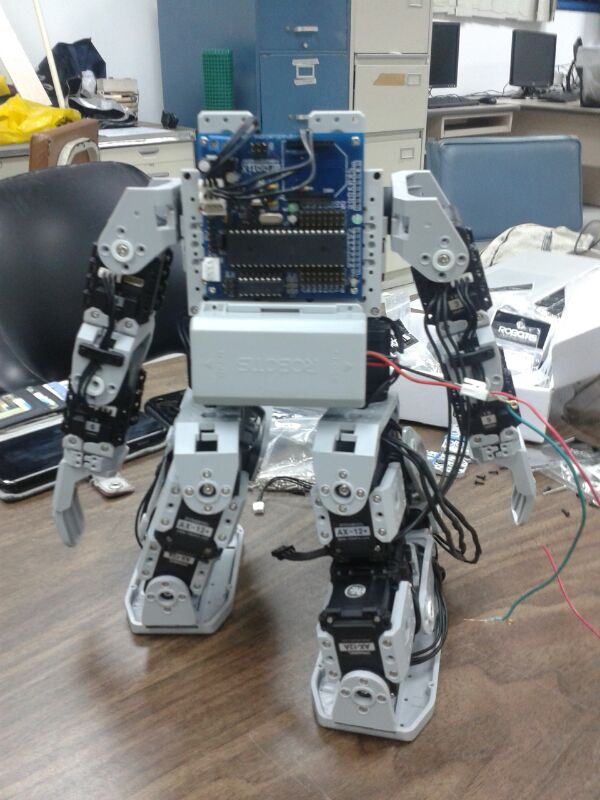
\includegraphics[height=05cm]{arbotixsola.jpg}
	\caption{  Parte trasera del robot con la Arbotix}
	\label{fig:figura1}
\end{figure}
\begin{figure}[ht!]
	\centering
		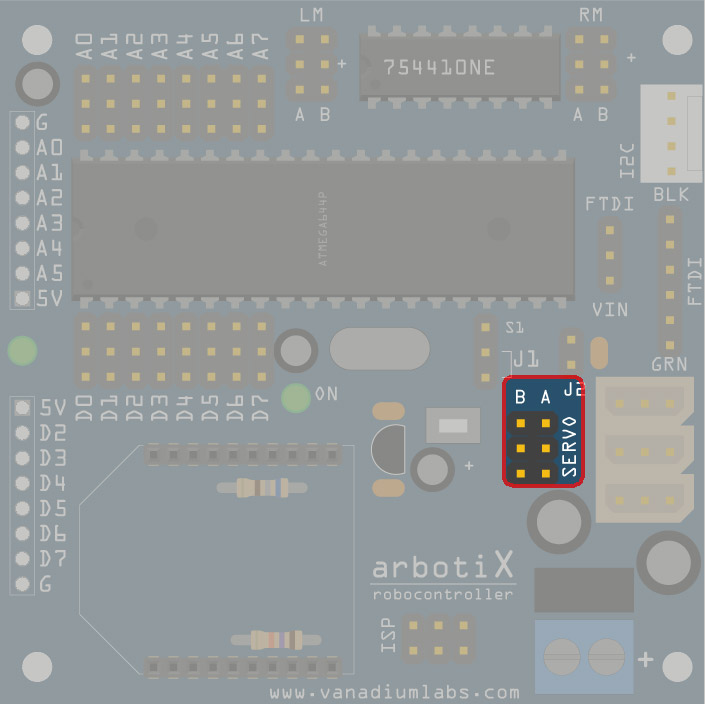
\includegraphics[height=05cm]{arbotix_hobby_servo.jpg}
		
    	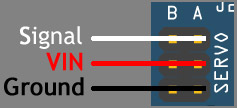
\includegraphics[height=2cm]{arbotix_hobbyservos_lines.jpg}
	\caption{  Ilustración de los puertos Hobby de la Arbotix
}
	\label{fig:figura2}
\end{figure}

\begin{figure}[ht!]
	\centering
		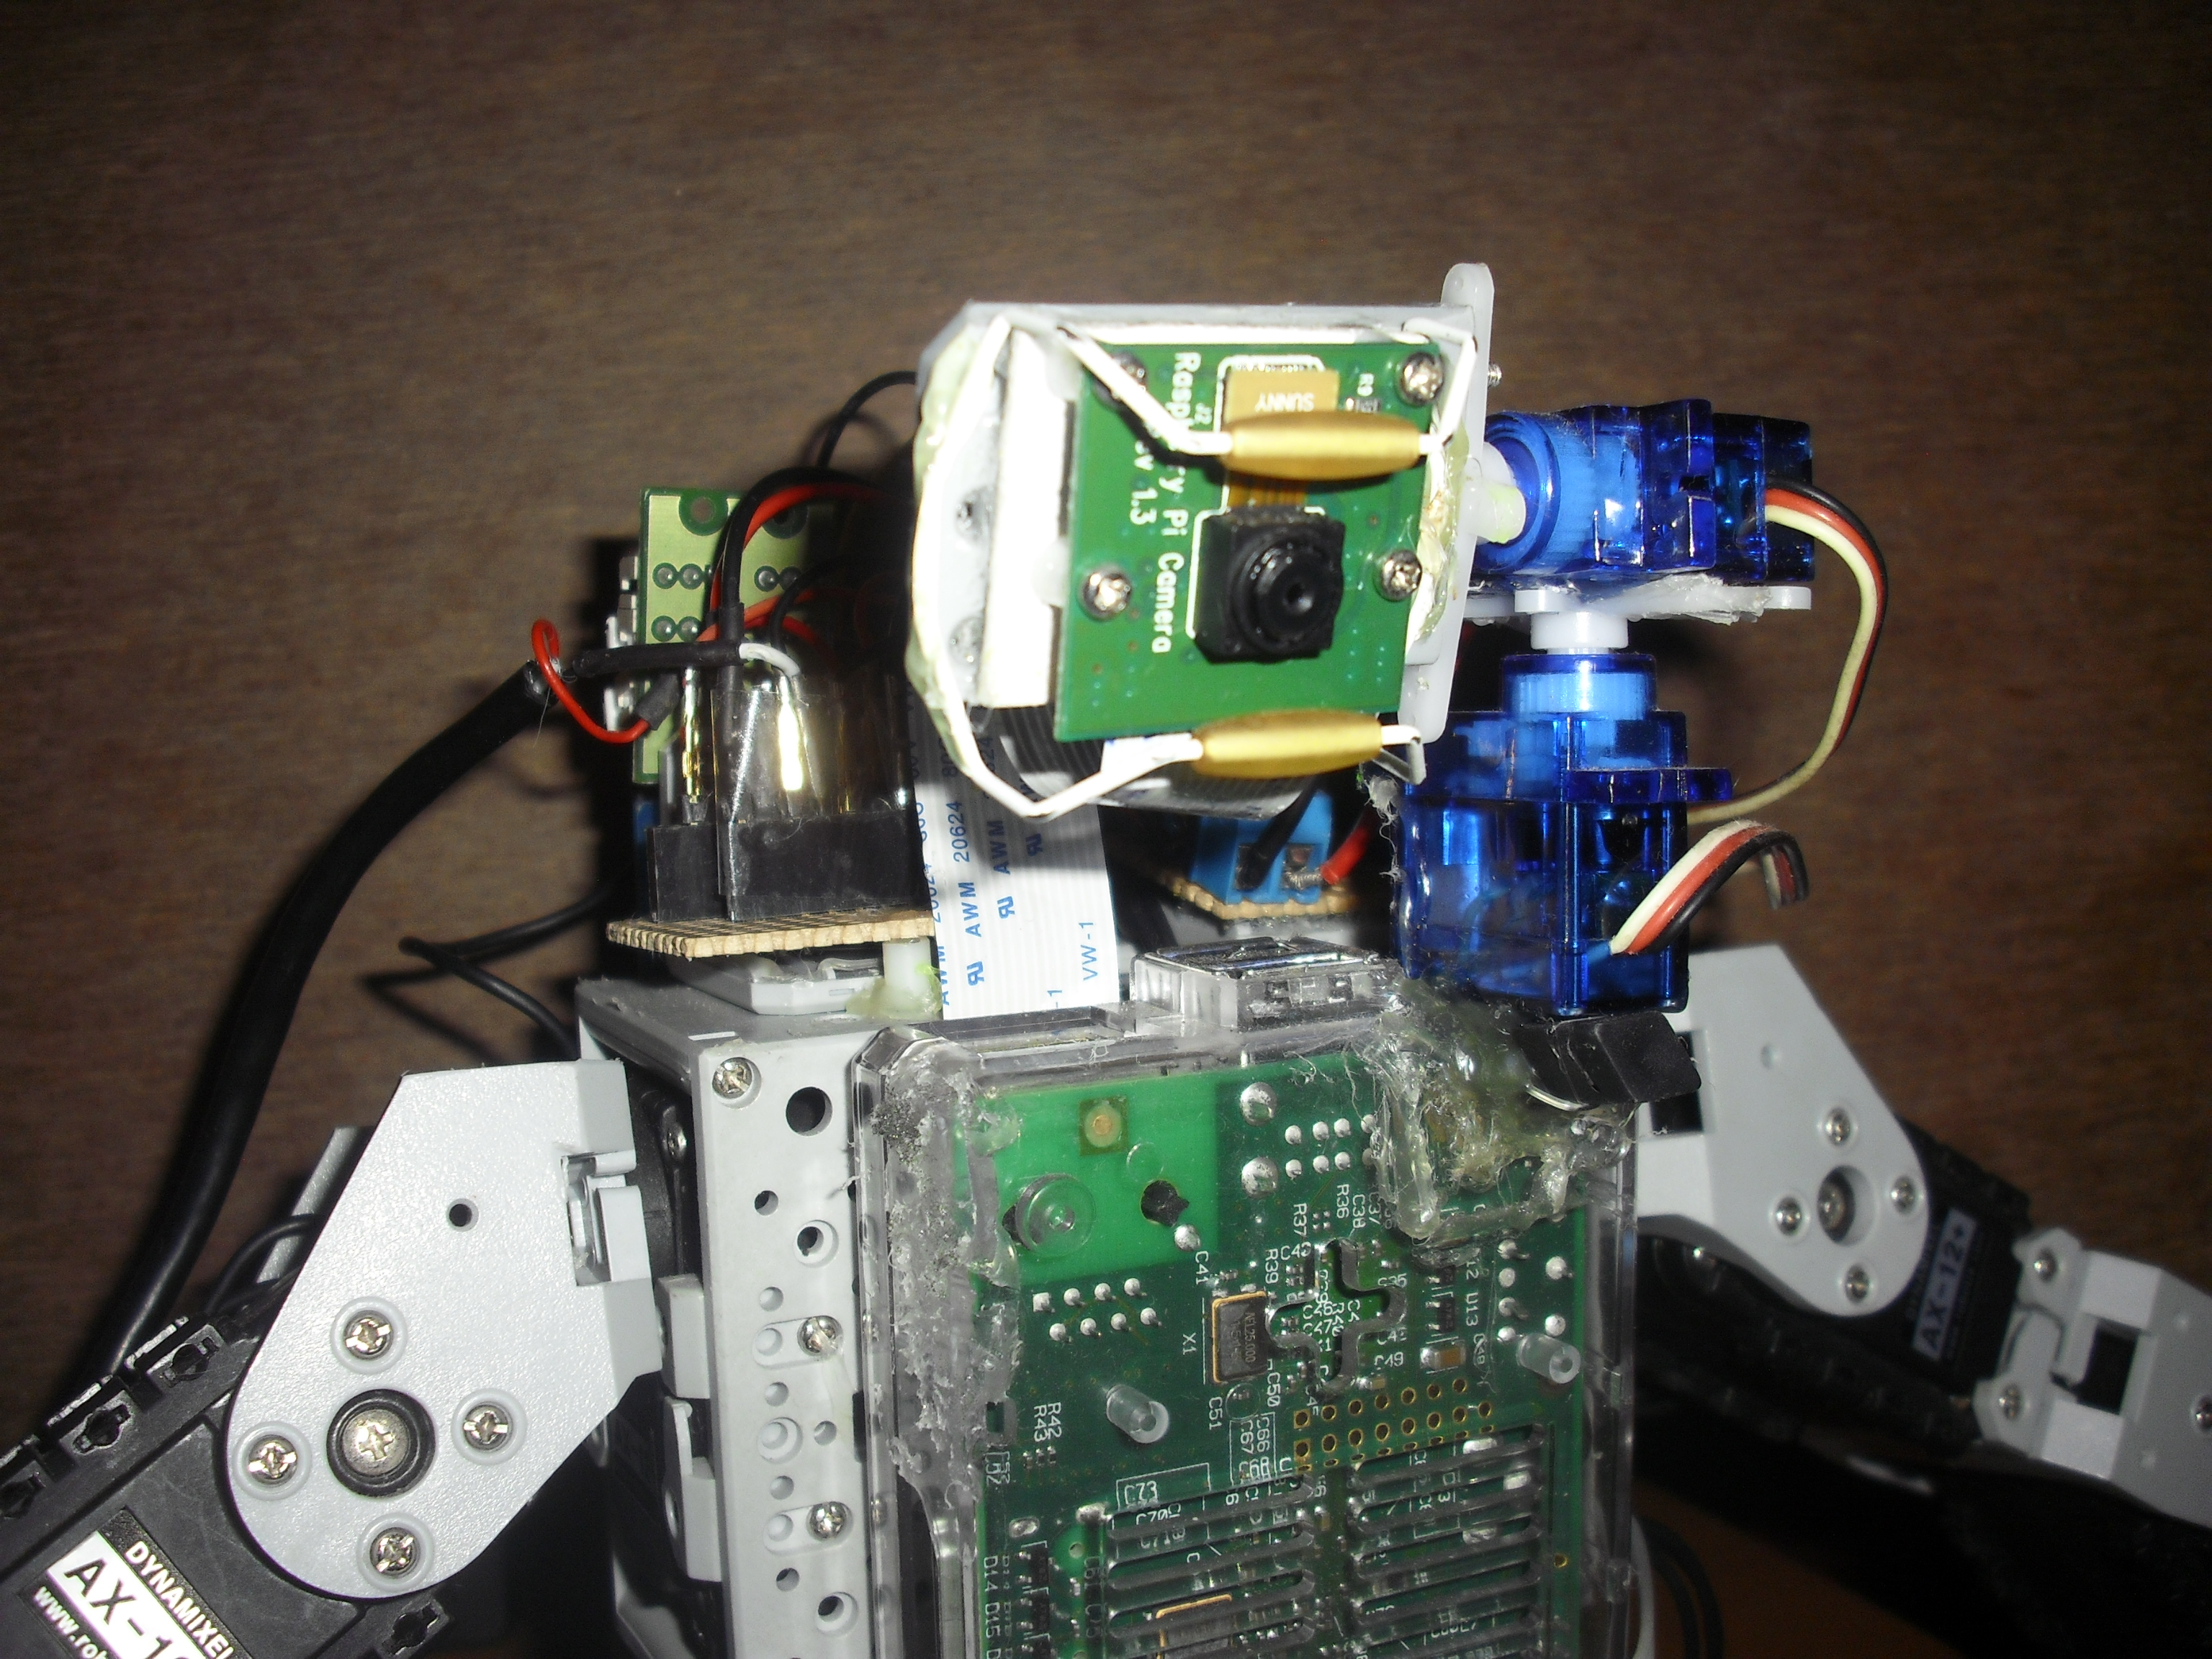
\includegraphics[height=05cm]{CIMG0025.JPG} 	
	\caption{ Vista delantera del robot con la cámara y servomotores instalados}
	\label{fig:figura3}
\end{figure}




En lugar de la utilización de la tarjeta CM-510 se ha decidido usar la tarjeta controladora Arbotix, particularmente en este proyecto el cambio se ha debido a que la controladora CM-510 no acepta la incorporación actuadores o dispositivos adicionales. La Arbotix permite la incorporación de nuevos actuadores y más dispositivos con sencillez, la programación, basada en el lenguaje Processing, se ha realizado bajo el IDE de Arduino. En la figura 1 se puede observar la estructura del robot con la Arbotix incorporada. En la parte interna del tronco del robot se sitúa el sensor Gyro. 

El movimiento de la cámara se ha logrado incorporando dos servomotores, uno para el movimiento horizontal y otro para el vertical. La conexión es pin a pin en los puertos especiales para ese tipo de motores (‘Hobby servo’) \cite{trossen} (ver figura 2). La cámara ha sido conectada a la Raspberry Pi en el puerto CSI. El resultado de estas tres piezas instaladas en el robot se puede apreciar en la figura 3.



%--------------------------------------------------------------------
\section{Movimiento}
\label{sec:movimiento}


Para que Debupa pueda cumplir sus objetivos debe ser capaz de ejecutar los siguientes movimientos:
\begin{itemize}
\setlength{\itemsep}{1pt}
\item Caminar hacia adelante
\item Girar a la izquierda
\item Girar a la derecha
\item Levantarse cuando ha caído boca abajo
\item Levantarse cuando ha caído boca arriba 
\item Patear con la pierna derecha e izquierda
\item Mover la cámara en sentido horizontal y vertical 

 
\end{itemize}

Se ha logrado realizar estos movimientos a través de la fijación de poses con la utilización del software Pypose, una aplicación para modelado de poses, que permite la lectura simultánea de las posiciones de todos los motores. De esta manera se ha fijado y guardado, para Debupa, un conjunto de poses necesarias para caminar, girar, patear y levantarse. Luego se ha podido generar en Pypose una secuencia de poses para cada movimiento. Finalmente se ha exportado el archivo de las poses y secuencias para ser utilizadas en el programa a ser ejecutado en Arbotix. 

Para detectar una posible caída del robot se ha incorporado el sensor giroscopio Gyro. Los valores de este sensor son leídos constantemente desde la Arbotix para corregir al robot en caso de una caída.  

\section{Experimentos de movimientos }
\label{sec:experimento}

\begin{figure}
\label{fig:experimento1}
\begin{tikzpicture}
    \begin{axis}[
        width  = 0.4*\textwidth,
        height = 8cm,
        major x tick style = transparent,
        ybar,
        bar width=10pt,
        ymajorgrids = true,
        ylabel = {Pruebas de Movimiento N=50},
        symbolic x coords={Ade,Der,Izq,PatearD,PatearI},
        xtick = data,
        scaled y ticks = false,
         legend style={at={(0,0)},anchor=north east,at={(axis description cs:0,-0.1)}}
    ]
        \addplot[style={bblue,fill=bblue,mark=none}]
            coordinates {(Ade, 49) (Der,50) (Izq,50) (PatearD,50) (PatearI,50)};

        \addplot[style={rred,fill=rred,mark=none}]
             coordinates {(Ade,1) (Der,0) (Izq,0)};
             
        \legend{Positivo ,Corrigió, Pateo}
    \end{axis}
  
  
\end{tikzpicture}

\caption{Experimento 1: Cantidad de veces que realiza acciones unitarias}
\end{figure}
Se realizaron varios experimentos para comprobar la movilidad del robot. Primero se debe definir los movimientos que representan una unidad. Cada una de las siguientes acciones constituyen una unidad: caminar hacia adelante (Ade) , girar hacia la derecha (Der), girar hacia la izquierda (Izq), patada con la pierna derecha (PatearD), patada con la pierna izquierda(PatearD), levantarse en la posición supino, levantarse en posición prono.

El primer experimento consistió en verificar la ejecución de las unidades de acciones, para ello se procedió a realizar la ejecución de cada unidad 50 veces, se tomó nota de las veces que lo realizaba de forma esperada (Positivo), y de aquellas que no lo hacía, si podría recuperarse de su mala acción (Corrigió) o no. Los resultados pueden observarse en la figura 4. En cuanto al balance del robot,  solo una vez se cayó, sin embargo, logró levantarse satisfactoriamente.

En el segundo experimento se evalu\'o la ejecuci\'on de  combinaciones de varias unidades de movimiento. Las combinaciones elegidas fueron: 

\begin{itemize}
\setlength{\itemsep}{1pt}
\item Caminar hacia adelante y patear con la pierna derecha (APD)
\item Caminar hacia adelante y patear con la pierna izquierda (API)
\item Caminar hacia adelante, girar hacia la derecha y patear con la pierna derecha (ADPD)
\item Caminar hacia adelante, girar hacia la derecha, patear con la pierna izquierda (ADPI)
\item Caminar hacia adelante, girar hacia la izquierda y patear con la derecha (AIPD)
\item Caminar hacia adelante, girar hacia la  izquierda y  patear con la pierna izquierda (AIPI)
\item Girar hacia la izquierda y patear con la pierna derecha (IPD)
\item Girar hacia la derecha y patear con la izquierda (DPI)
\item Girar hacia la derecha y patear con la pierna derecha (DPD)
\item Girar hacia la izquierda y patear con la pierna izquierda (IPI)
 \end{itemize}


Se realizaron 30 pruebas de cada una de estas combinaciones. Los resultados se han dividido en dos gr\'aficos (figuras 5 y 6) para mejorar su visualizaci\'on.  En el peor caso (ADPD),  Debupa logra patear la pelota 26 de las 30 veces al final del movimiento combinado. El robot s\'olo se ha ca\'ido dos veces, pero ha logrado levantantarse con \'exito (figura 5).


%\begin{tabular}{|c|c|}
%\hline 
%Ade & Caminar hacia adelante \\ 
%\hline 
%Der & Girar hacia la derecha \\ 
%\hline 
%zq & Girar hacia la izquierda \\ 
%\hline 
%PatearD & Patear conla derecha \\ 
%\hline 
%PatearI & Patear con la izquierda \\ 
%\hline 
%\end{tabular} 

\begin{figure}[th!]
\begin{tikzpicture}
    \begin{axis}[
        width  = 0.4*\textwidth,
        height = 8cm,
        major x tick style = transparent,
        ybar,
        bar width=8pt,
        ymajorgrids = true,
        ylabel = {Pruebas de Movimiento N=30},
        symbolic x coords={APD, API, ADPD,ADPI, AIPD},
        xtick = data,
        scaled y ticks = false,
         legend style={at={(0,0)},anchor=north east,at={(axis description cs:0,-0.1)}}
    ]
        \addplot[style={bblue,fill=bblue,mark=none}]
            coordinates { (APD,29) (API,30)(ADPD,30)(ADPI,30)(AIPD,29)};

        \addplot[style={rred,fill=rred,mark=none}]
             coordinates { (APD,1) (AIPD,1)};

        \addplot[style={ggreen,fill=ggreen,mark=none}]
             coordinates { (APD,30) (API,27)(ADPD,26)(ADPI,30)(AIPD,29)};
    
    
        \legend {Positivo,Corrigió,Pateó}
    \end{axis}
\end{tikzpicture}
\caption{Experimento 2.a: Veces que realiza acciones combinadas}
\end{figure}


\begin{figure}[th!]
\begin{tikzpicture}
    \begin{axis}[
        width  = 0.4*\textwidth,
        height = 8cm,
        major x tick style = transparent,
        ybar,
        bar width=8pt,
        ymajorgrids = true,
        ylabel = {Pruebas de Movimiento N=30},
        symbolic x coords={  AIPI, IPD, DPI, DPD,IPI},
        xtick = data,
        scaled y ticks = false,
         legend style={at={(0,0)},anchor=north east,at={(axis description cs:0,-0.1)}}
    ]
        \addplot[style={bblue,fill=bblue,mark=none}]
            coordinates { (AIPI,30)(IPD,30)(DPI,30)(DPD,30)(IPI,30)};

        \addplot[style={rred,fill=rred,mark=none}]
             coordinates {(AIPI,0) };

        \addplot[style={ggreen,fill=ggreen,mark=none}]
             coordinates { (AIPI,28) (IPD,30)(DPI,30)(DPD,30)(IPI,30)};
        
        \legend {Positivo,Corrigió ,Pateo}
    \end{axis}
\end{tikzpicture}
\caption{Experimento 2.b: Veces que realiza acciones combinadas}
\end{figure}



%---------------------------------------------------------------------------------------------------------
\section{Detección}
\label{sec:deteccion}


En esta sección se presentan las herramientas y estrategias con las cuales se ha abordado el problema de la detección de la pelota.

\subsection{Integrando la Raspberry Pi y la cámara}
Se ha incorporporado un mini computador Raspberry Pi 2011.12 y una cámara Raspberry Pi 1.3 que actúe como “los ojos” del robot y así lograr obtener un modelo parcial del ambiente. La cámara ha sido instalada sobre dos servo-motores RC, otorgándole dos grados de libertad y un rango visibilidad de 160 grados en una posición fija del robot.

Estos motores se controlan desde la Arbotix usando la librería HServo \cite{vanadium}, que aunque sólo puede ser usada para los motores conectados en los puertos Hobby (12 y 13), brinda la ventaja de un control más preciso, evitando que los motores tiemblen. 
 

\subsection{Detección de la pelota con openCV}
Para lograr conocer la ubicación de la pelota en un momento dado y de forma autónoma se ha decidido aplicar detección por ‘blobs’, o reconocimiento de regiones, esta técnica consiste en filtrar la imagen por color. Por ello es importante que el color de la pelota no se repita en el ambiente y así poder obtener la posición de la pelota dentro de la imagen. Se han utilizado las librerías de OpenCV para apoyar esta tarea.

Los filtros o transformaciones aplicadas han sido la morfología en apertura y en clausura. La morfología en apertura es una transformación de una imagen que consiste en aplicar la operación de erosión seguida de la operación de dilatación \cite{filtros}. La morfología de clausura es una transformación que aplica la dilatación seguida de la erosión.


El resultado de estos filtros es una imagen en blanco y negro, derivada de la imagen original, en la que se identifica con blanco el rango de valores establecido del color que se requiere buscar y el resto de la imagen en negro. 

\subsection{Discretización de la imagen y acciones del robot}

El hecho de  que la cámara tenga dos grados de libertad para moverse es una gran ventaja, ya que se puede obtener un mayor rango de visión. Debupa puede mirar hacia la derecha o izquierda sin tener que mover sus pies, también puede mirar hacia abajo para verificar que la pelota esté en sus pies, para patear, o hacia arriba para ubicar la pelota a mayor distancia. La desventaja es que agrega mayor complejidad.

Debupa debe tomar una acción diferente dependiendo de la posición de la cámara y de la pelota en la imagen. Sin embargo esto genera una gran cantidad de estados, por lo cual se ha decidido discretizarlos de la siguiente manera:  
\begin{itemize}
\item La cámara tiene 9  (3x3) posibles posiciones. La visión horizontal abarca 3 cuadros, aproximadamente 160 grados. La visión vertical también abarca 3 cuadros, llega a captar la imagen desde sus pies hasta más de 2 metros hacia adelante.
\item Desde cada posición de la cámara se obtiene una imagen y, dependiendo de la posición, la imagen se divide en diferentes regiones. 
\end{itemize}
 
Las im\'agenes de la c\'amara obtenidas en la posici\'on central, y en la posicio\'n central inferior son las m\'as importantes y prioritarias, pues si la pelota se detecta en ellas significa que el robot est\'a cerca de poder patearla. Estas dos im\'agenes se dividen en las regiones que pueden ser apreciadas en la figura 7. Cada región ayuda a identificar la acción que Debupa debe tomar. Por ejemplo, en el cuadro central inferior, cuando la pelota se encuentra del lado derecho de la pantalla (región 13 o 17) el robot debe girar a la derecha para situarse de frente a la pelota. El \'area de pateo se encuentra en las regiones 15 y 16.

\begin{figure}
 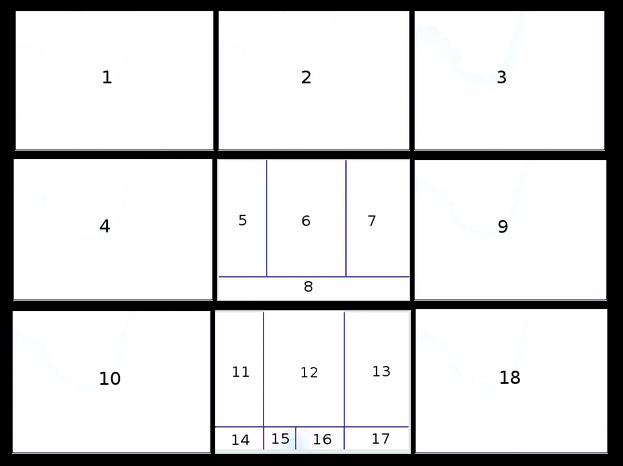
\includegraphics[height=6cm]{discretizacion.png}
 \caption{Campo de visión del robot con el número de cada región}
 	\label{fig:figura4}
 \end{figure} 

%\subsection{Acciones del robot en función de la ubicación de la pelota}

A continaci\'on se especifica la acción a tomar en cada región:

\begin{itemize}
\item Girar a la Izquierda: Debupa debe girar a la izquierda cuando la pelota se encuentre en alguna de las siguientes regiones: 1, 4, 10, 5, 11, 14.

\item Girar a la Derecha: debe girar a la derecha cuando la pelota se ubique en alguna de las siguientes regiones: 7, 13, 17, 3, 9, 18. 

\item Caminar hacia adelante: cuando la pelota se ubique en alguna de las siguientes regiones: 12, 6, 2.

\item Patear con la pierna izquierda: cuando la pelota se encuentre en la región 15.

\item Patear con la pierna derecha: cuando la pelota se encuentre en la región 16.
\end{itemize}
%--------------------------------------------------------------------------------------------------------------------

\section{Integración de los componentes }
\label{sec:integracion}
La Raspberry Pi procesa la información de la cámara y la Arbotix controla los actuadores. Para coordinar los movimientos del robot según la posición de la pelota se ha establecido una forma de comunicación entre ambas tarjetas. 

Se seleccionado la Arbotix como servidor de peticiones y a la Raspberry Pi como cliente. Dentro de la Raspberry Pi se ejecuta el proceso de decidir qué acción debe tomar el robot. Una vez determinada la acción se envía la petición a la Arbotix para que esta la ejecute. Este proceso es  bidireccional y síncrono, es decir, la Raspberry envía la petición y se bloquea hasta que la Arbotix retorne la respuesta de su culminación.  

Para la implementación de la comunicación se ha usado ROS (Robot Operating System) con la utilización de los servicios que no es más que un método de comunicación basado en el paradigma de request/reply con el concepto de maestro esclavo.
\section{Experimentos con comportamientos integrados}
\label{sec:experimentosintegrados}

El experimento 3 consiste en pruebas de desempeño donde se observa el comportamiento global del robot con todos sus componentes integrados. El  primer caso (Caso1) consiste en la colocación de la pelota  en la zona de pateo  (las regiones 15 y 16 de la figura 7). El número de pruebas en este primer caso fue de 10, cuya duración aproximada de cada prueba fue de 30 segundos.
El segundo caso  (Caso2) consistió en en la colocación inicial de la pelota a una distancia de 50 cm en línea recta al robot. Se realizaron 10 pruebas, siendo la duración aproximada de 2 minutos en cada una. 

La figura 8 muestra los resultados experimentales.  Se registra si el robot ubica la posición de la pelota (Detecta), se sitúa al frente de ella  (Llega) y patea la pelota con éxito (Patea). Para el caso 1 el desempeño del robot fue favorable ya que en un 90\% de los casos completó la prueba satisfactoriamente logrando patear la pelota. Para el caso 2 Debupa logró cumplir la tarea asignada en un 50\% del número de pruebas ejecutadas, determinando que la estrategia se podría mejorar sustancialmente.



\begin{figure}
\begin{tikzpicture}
    \begin{axis}[
        width  = 0.4*\textwidth,
        height = 8cm,
        major x tick style = transparent,
        ybar,
        bar width=10pt,
        ymajorgrids = true,
        ylabel = {Pruebas de Desempeño N=10},
        symbolic x coords={Caso1,Caso2},
        xtick = data,
        scaled y ticks = false,
         legend style={at={(0,0)},anchor=north east,at={(axis description cs:0,-0.1)}}
    ]
        \addplot[style={bblue,fill=bblue,mark=none}]
            coordinates {(Caso1, 9) (Caso2,7) };

        \addplot[style={rred,fill=rred,mark=none}]
             coordinates {(Caso1,9) (Caso2,5) };
        \addplot[style={ggreen,fill=ggreen,mark=none}]
             coordinates {(Caso1,9) (Caso2,5) };
             
        \legend{Detecta ,Llega, Pateo}
    \end{axis}
  
\end{tikzpicture}

\caption{Experimento 3: Desempe\~no de movimientos integrados}
\end{figure} 

\section{Consideraciones especiales}
\label{sec:consideraciones}

El uso de los motores Dynamixel Ax-12+ debe ser cuidadoso dado que por el exceso de esfuerzo, si no se controla la temperatura máxima o el torque máximo permitido, suelen quemarse con facilidad. El sensor de temperatura es capaz de medir valores entre -5\celsius~y 80\celsius, y el torque puede ir desde 512 hasta 1023 kgf-cm. La solución aplicada ha sido establecer en el chip de cada motor una cota máxima de 30\celsius~ de temperatura y un torque máximo de 800 kgf-cm. En caso de superar alguna de estas cotas los motores se apagan automáticamente evitando así un daño mayor. Para lograr esto se ha tenido que modificar la librería Ax12 agregando algunos procedimientos que permitieran establecer la temperatura y el torque máximo.

Para ampliar información sobre este proyecto se encuentra disponible el blog de Debupa en donde se presenta la descripción de algunas de las tareas que han presentado problemas con sus soluciones (\url{ https://sites.google.com/site/arbotixml3j/home}).


\section{Conclusiones}
\label{sec:Conclusiones}

La presente investigación ha nacido de la motivación por hacer que en Venezuela se incursione en proyectos que involucren humanoides autónomos e inteligentes. Se ha inspirado especialmente en la categoría Robocup soccer de la competencia internacional Robocup. Desde 1997, fecha en la que inició la competencia, Venezuela nunca ha participado en categorías con humanoides, mientras que países latinoamericanos como México, Brasil y Colombia sí han tenido avances en este campo. Si bien este proyecto no cumple con todas las reglas de la competencia se espera que éste pueda dar pie a continuar investigaciones dentro de Venezuela. 

Los componentes utilizados en este proyecto son relativamente económicos comparados con otros en el mercado. La integración del kit Bioloid Premium con la Arbotix y la Raspberry Pi, ha hecho posible construir un humanoide inteligente sin tener que invertir exorbitantes cantidades de dinero. Una de las contribuciones más importantes es la coordinación y paralelismo exitoso entre todos los componentes utilizados.

Las mejoras que se pueden incorporar al proyecto podrían ser: la inclusión de aprendizaje por reforzamiento para patear de forma exitosa, incluir que la patada sea en dirección al arco e incluso añadir aprendizaje por reforzamiento para hacer que el robot pueda predecir la posición de una pelota en movimiento para que pueda patearla en el momento indicado.  


% Utilice el archivo MCIng2014.bib para incluir sus referencias bibliográficas:
\bibliography{referencias}
\bibliographystyle{ieeetran}


% that's all folks
\end{document}


